%%% XProbes Docs
%%%
%%% http://www.iks.it
%%% Internal procedural guides
%%% 07/2014

%%%%% Preamble
% KOMA scrartcl is called for several reasons:
%   Nicer page margins without the need of the 'geometry' package
%   Perfectly fitting abstract environment
%   High customizability
\documentclass[11pt,a4paper]{scrartcl}
%%%%%%%% Per code java
\usepackage{listings}
\usepackage{color}

\definecolor{dkgreen}{rgb}{0,0.6,0}
\definecolor{gray}{rgb}{0.5,0.5,0.5}
\definecolor{mauve}{rgb}{0.58,0,0.82}

\lstset{frame=tb,
  language=Java,
  aboveskip=3mm,
  belowskip=3mm,
  showstringspaces=false,
  columns=flexible,
  basicstyle={\small\ttfamily},
  numbers=none,
  numberstyle=\tiny\color{gray},
  keywordstyle=\color{blue},
  commentstyle=\color{dkgreen},
  stringstyle=\color{mauve},
  breaklines=true,
  breakatwhitespace=true,
  tabsize=3
}
\lstset{language=Java}




%%% Packages %%%
\usepackage[latin1]{inputenc}
\usepackage{amsmath,amsfonts,amssymb}  % Math packages
\usepackage{multicol}
%%% URLs
\usepackage{hyperref}
%%% Graphics
\usepackage{graphicx}
%%% Colors & graphics
\usepackage[table]{xcolor}
\usepackage{color}
\usepackage{graphicx}
\usepackage{float}
\usepackage{caption}
\usepackage{longtable}

%%% Code Listing
\usepackage{listings}
%%% URLs
\usepackage{hyperref}

%%% Framed
\usepackage{framed}
\usepackage{mdframed}

\usepackage{caption}
\captionsetup[lstlisting]{font={small}}

%%% Define colors
\definecolor{dkgreen}{rgb}{0,0.6,0}
\definecolor{gray}{rgb}{0.5,0.5,0.5}
\definecolor{mauve}{rgb}{0.58,0,0.82}
\definecolor{lightblue}{rgb}{0.68, 0.85, 0.9}

\lstset{frame=tb,
  escapeinside={(*}{*)},%
  language=bash,
  aboveskip=3mm,
  belowskip=3mm,
  showstringspaces=false,
  columns=flexible,
  basicstyle={\small\ttfamily},
  numbers=left,
  numberstyle=\tiny\color{gray},
  commentstyle=\color{dkgreen},
  stringstyle=\color{mauve},
  breaklines=true,
  breakatwhitespace=true,
  postbreak=\raisebox{0ex}[0ex][0ex]{\ensuremath{\color{red}\hookrightarrow\space}},
  tabsize=3,
  keywords=[2]{GET, POST, DELETE, UPDATE, PATCH},
  keywordstyle={[2]\color{blue}}
}


%%%%%%%%%%%%%%%%%%%%%%%%%
%%%%%% Definitions %%%%%%
%%%%%%%%%%%%%%%%%%%%%%%%%
%%% Define a new command that prints the title only
\makeatletter       % Begin definition
\def\printtitle{	% Define command: \printtitle
    {\centering \huge \normalfont \textbf{\@title}\par}}	% Typesetting
\makeatother		% End definition

%%% Global vars for the doc	
\newcommand{\projectName}{Project\registered{}}
\newcommand{\companyName}{XTN : Stage Univerit\`a di Padova}
\newcommand{\docName}{Base di Dati a Grafo in ambito antifrode}
\newcommand{\versionNum}{1.0}
\newcommand{\termine}[1]{\textit{#1}\small{$_G$}}
\renewcommand{\url}[2]{\href{#2}{\textcolor{blue}{\texttt{#1}}}}
\newcommand{\link}[1]{\href{#1}{\textcolor{blue}{\texttt{#1}}}} 


% apiversion defines the MORE API Version in URL Scheme
% this MUST be changed when updating the API to a new verion.
\def \apiversion {3}

%%%%%%%%%%%%%%%%%%%%%%%%%
%%% Disclosure Policy %%%
%%%%%%%%%%%%%%%%%%%%%%%%%
\newcommand{\secretDoc}{~}
\newcommand{\privateInternalDoc}{X}
\newcommand{\privateBusinessDoc}{~}
\newcommand{\publicDoc}{~}
\newcommand{\registered}{$^{\scriptsize\mathrm{\textregistered{}}}$}
\newcommand{\ident}[1]{\textit{#1}}
\newcommand{\method}[1]{\textbf{#1}}
\newenvironment{request}[1]{\begin{mdframed}[backgroundcolor=black!5,linecolor=red!60!black,linewidth=2pt,topline=false,
  rightline=false,
  bottomline=false,innertopmargin=8pt,innerbottommargin=6pt] \method{#1}~}{\end{mdframed}}
\newcommand{\paramex}[1]{\textcolor{mauve}{\texttt{#1}}}
\newcommand*\pct{\scalebox{.8}{\%}}

\title{Base di Dati a Grafo in ambito antifrode}

%%% Define a new command that prints the author(s) only
\makeatletter           % Begin definition
\def\printauthor{       % Define command: \printauthor
    {\large \@author}}  % Typesetting
\makeatother            % End definition

\author{
	Luca Dario \\
	\companyName \\
	\texttt{luca.dario29@gmail.com}\vspace{40pt} \\
    }

%%%%%%%%%%%%%%%%%%%%%%%%%
%%% Header and footer %%%
%%%%%%%%%%%%%%%%%%%%%%%%%
\usepackage{fancyhdr}  % Needed to define custom headers/footers
	\pagestyle{fancy}  % Enabling the custom headers/footers
\usepackage{lastpage}	

% Header (empty)
\lhead{
\includegraphics[scale=0.55]{xtn}}
\chead{}
\rhead{\projectName~ - ~\docName}
% Footer (you may change this to your own needs)
\lfoot{\footnotesize \companyName \\
    Headquarter: Arco (TN), via Santa Caterina 95 - 38062 \\
    Executive Office: Rovereto (TN), C.so Rosmini, 8 - 38068 \\
    +39 049 870 10 10 (phone) \textbullet ~+39 049 870 10 14 (fax) \\
    info@xtn-lab.com \textbullet ~www.xtn-lab.com \\
    P.I \textbullet ~C.F. \textbullet ~Reg. Imprese 04395340286
}
\cfoot{}
\rfoot{\footnotesize page \thepage\ of \pageref{LastPage}}	% "Page 1 of 2"
\renewcommand{\headrulewidth}{0.2pt}
\renewcommand{\footrulewidth}{0.2pt}

%%% Change the 'KOMA' sectioning fonts back to standard LaTeX font (this is just a matter of taste)
\setkomafont{sectioning}{\rmfamily\bfseries\boldmath}

%%% Change the abstract environment
\usepackage[runin]{abstract}        % runin option for a run-in title
\setlength\absleftindent{10pt}      % left margin
\setlength\absrightindent{10pt}     % right margin
\abslabeldelim{\quad}				 
\setlength{\abstitleskip}{-10pt}
\renewcommand{\abstracttextfont}{\small \slshape}	% slanted text
\usepackage[latin1]{inputenc}
\usepackage{eso-pic}
\newcommand\BackgroundPic{%
    \put(0,0){%
        \parbox[b][\paperheight]{\paperwidth}{%
            \vfill
            \centering
            
\includegraphics[width=\paperwidth,height=\paperheight,%
            keepaspectratio]{page_background.png}%
            \vfill
        }
    }
}

%%%%%%%%%%%%%%%%%%%%%%%%%
%%%% Document start %%%%%
%%%%%%%%%%%%%%%%%%%%%%%%%
\begin{document}

\AddToShipoutPicture*{\BackgroundPic} %%% without * replicate on all pages

%%% Top of the page: Author, Title and Abstact
\begin{minipage}[t]{0.35\linewidth}
	\begin{flushright}
		\printauthor
	\end{flushright}
\end{minipage} \hspace{0pt}
%
\begin{minipage}[b]{0.02\linewidth}
	%%\rule{3pt}{175pt}
	\rule{0pt}{175pt}
\end{minipage} \hspace{0pt}
%
\begin{minipage}[t]{0.63\linewidth}
%\begin{flushleft}
\printtitle 
\vspace{5pt}
	\begin{abstract} 
Questo documento descrive il processo di analisi delle varie tecnologie, che utilizzano base di dati a grafo, e il successivo sviluppo del Poc.
	\end{abstract}
%\end{flushleft}
\end{minipage}
\vspace{20pt}       % Add some vertical spacing to separate the abstract from the rest of the article

\pagebreak % NEWPAGE FOR AESTHETICS

%%% TABLE OF CONTENTS
\tableofcontents
\pagebreak % NEWPAGE FOR AESTHETICS

%%% METADATA
\section{Metadata}
These section reports all info about this document.

\subsection{Scope}

\begin{center}
    \raggedright
    \begin{tabular}{| l | l |}
    \hline
    SECRET & \secretDoc\\
    \hline
    PRIVATE INTERNAL USE & \privateInternalDoc\\
    \hline
    PRIVATE BUSINESS USE & \privateBusinessDoc\\
    \hline
    PUBLIC & \publicDoc\\
    \hline
    \end{tabular}
\end{center}
The information contained herein are privileged and confidential. If you are not the intended recipient, please contact the sender and delete this document. Any unauthorised copying of this document or unauthorised distribution of the information is strictly prohibited.
\bigskip

\subsection{Version and Revisions}

Authoring history:
\begin{center}
    \raggedright
    \begin{tabular}{|p{3cm}|p{3cm}|p{3.5cm}|p{2cm}|}
    \hline
    \textit{Version number} & \textit{Author} & \textit{Team} & \textit{Date} \\
    \hline  0.1 & Luca Dario & \companyName & 31/10/17 \\
    \hline
    \end{tabular}
\end{center}

Review history:
\begin{center}
    \raggedright
    \begin{tabular}{|p{3cm}|p{3cm}|p{3.5cm}|p{2cm}|}
    \hline
    \textit{Review version} & \textit{Author} & \textit{Team} & \textit{Date} \\
    \hline    1.0 & ~ & \companyName & ~ \\
    \hline
    \end{tabular}
\end{center}

Approved by:
\begin{center}
    \raggedright
    \begin{tabular}{|p{3cm}|p{3cm}|p{2cm}|p{2cm}|}
    \hline
    \textit{Approved by} & \textit{Team} & \textit{Date} \\
    \hline ~ & ~ & ~ \\
    \hline
    \end{tabular}
\end{center}

\pagebreak % NEWPAGE FOR AESTHETICS

%%%%%%%%%%%%%%%%%%%%%%%%%%%%
%%% SECTION INTRODUCTION %%%
%%%%%%%%%%%%%%%%%%%%%%%%%%%%
\section{Introduzione}
Questo documento descrive le scelte che mi hanno portato alla decisione delle tecnologie di base di dati a grafo pi\'u valide, in ambito antifrode.
Dopo la fase di analisi il documento si focalizzer\'a nell'architettura del PoC sviluppato.

\pagebreak % NEWPAGE FOR AESTHETICS

%%% INLINE APIs %%%
\section{Alternative Tecnologiche}
\subsection{Introduzione}
La racconta delle informazioni necessarie alla scelta sono state reperite in primo luogo dalle documentazioni ufficiali delle case produttrici, successivamente dai forum quali StackOverflow, DZone.
Grazie ad una riunione con il mio Tutor aziendale, Giuseppe Pavan, sono stati decisi i seguenti punti di interesse per focalizzare l'analisi tecnologica.
\begin{itemize}
\item{Licenza:} verificare che tipo di licenza ha il prodotto e sopratutto se ha una versione gratuita e che tipo li limitazioni ha rispetto a quella a pagamento.
\item{Tipo:} verificare il tipo di tecnologia implementa, se una base di dati a grafo \termine{nativa} o non nativa.
\item{Modelli disponibili:} verificare che tipi di \termine{Modelli} offre questa tecnologia.
\item{Community:} verificare l'ampiezza di community del prodotto in analisi, se un prodotto ha una community molto sviluppata \'e possibile ricercare consigli o risoluzioni di determinati problemi nei vari forum di riferimento.
\item{Tecnologie sopportate nativamente(di rilievo per l'azienda):} verificare se la tecnologia mette a disposizione un supporto a tecnologie di riferimento all'azienda quali Java, Spring.
\item{Linguaggio di quering proprietario:} verificare se la tecnologia in analisi mette a disposizione un linguaggio di quering proprietario e ottimizzato per essa, analizzando la sua espressivit\'a.
\item{Supporto Tinkerpop:} verificare se la tecnologia mette a disposizione il supporto ad Apache \termine{tinkerpop}, sfruttando quindi un interfaccia comune permettendo poi un passaggio ad un altra tecnologia che lo supporta a costi nulli.
\item{Clustering:} verificare se la tecnologia mette a disposizione un sistema di clustering pronto all'uso, che tipo di clustering e se ha la possibilit\'a di eseguire query distribuite ed infine se questa \'e disponibile nelle versione gratuita.
\item{Security:} verificare che sistemi di sicurezza dei dati la tecnologia mette a disposizione e se \'e possibile dividere il database in zone per farle diventare accessibili solo a determinati utenti.
\end{itemize}
\subsection{\url{Sparksee(DEX)}{http://www.sparsity-technologies.com}:}
Sparksee \'e un database a grafo \termine{nativo} \termine{full ACID} scritto in C++ sviluppato da \url{Sparsity Technologies}{http://www.sparsity-technologies.com} a fine 2008 sotto nome "DEX" e successivamente, nel 2014, cambia il suo nome in Sparksee.\\
Sparksee \'e il primo database a grafo disponibile per Android ed iOS.
Ad oggi sia la versione desktop che mobile sono alla 5.2.
\begin{itemize}
\item \textbf{Licenza:} commerciale a pagamento, disponibile quella gratuita esclusiva per la valutazione o per fini accademici limitata a 1 milione di nodi.
\item \textbf{Tipo:} database multi grafo, Full ACID ed orientato di tipo nativo, con la possibilit\'a di aggiungere un numero illimitato di etichette sia sui nodi che sugli archi.
\item \textbf{\termine{Modelli} disponibili:} disponibile solamente \termine{modello a grafo}.
\item \textbf{Community:} molto bassa data la bassa diffusione a livello mondiale.
\item \textbf{Tecnologie supportate nativamente(di rilievo per l'azienda):} Java, Maven, C++ e disponibile per Linux, Windows, MacOS, iOS, Android, BB10.
\item\textbf{Linguaggio di quering proprietario:} API proprietarie disponibili per Java,C++,Phyton.
\item\textbf{Supporto \termine{Tinkerpop}:} Si.

\item\textbf{Clustering:} feauture gratuita ma molto approssimativa visto che in caso di malfunzionamento del master tutto il sistema andrebbe in down, oppure se, durante un operazione di scrittura, uno slave dovesse avere un malfunzionamento il master resterebbe in una sorta di limbo per un tempo infinito ad aspettare, inutilmente, l'avvenuta scrittura dal parte dello stesso slave. Le richieste di scrittura le riceve solo il master che, esso, le inoltrer\'a agli slave, invece quelle di lettura vengono ricevute da tutti gli slave.
\item\textbf{Security:} Non specificata nella loro documentazione e non travata in nessun forum.
\item\textbf{Monitoring:} \'e possibile attivare la registrazione e memorizzazione dei log e warning, statistiche come size del database, sessioni attive tempo di attivit\'a.
\item\textbf{Qualit\'a secondo la casa produttrice e informazioni aggiuntive:} 
\begin{itemize}
\item\textbf{Alta compressione:} la casa produttrice promette di "minimizzare" lo spazio occupato dal database grazie all'alta velocit\'a di compressione data struttura rappresentata in bitmap. Ogni dato \'e rappresentato solo una volta, evitando repliche inutili.
\item\textbf{I/O efficiente:} ciascuna delle bitmap \'e partizionata in blocchi per migliorare la localizzazione I/O.
\end{itemize}
\end{itemize}
\newpage



\subsection{\url{Neo4j}{https://neo4j.com/}}
Neo4j \'e un software per base di dati a grafo \termine{nativo}, \termine{full ACID}, sviluppato in Java dalla Neo Technology  nel 2007.
E' il software del suo genere pi\'u usato al mondo ed \'e usato da multinazionali come Microsoft, AirBnb, IBM, Ebay.
Attualmente \'e alla versione 3.2.4.
Ad oggi sia la versione desktop che mobile sono alla 5.2.
\begin{itemize}
\item \textbf{Licenza:} GNU GPL v3 con versione interprise a pagamento. La versione gratuita non ha limiti sulla dimensione del database ma la versione interprise aggiunge il supporto al crustering, la versione embedded e supporto 24/7.
\item \textbf{Tipo:} database multi grafo, Full ACID ed orientato di tipo nativo, con la possibilit\'a di aggiungere un numero illimitato di etichette sia sui nodi che sugli archi.
\item \textbf{\termine{Modelli} disponibili:} disponibile solamente \termine{modello a grafo}.
\item \textbf{Community:} essendo il software per database a grafo pi\'u diffuso ha una community relativamente molto ampia.	
\item \textbf{Tecnologie supportate nativamente(di rilievo per l'azienda):} Java, Maven, Spring Data Neo4j, Phyton per quanto riguarda la versione server tramite REST, invece la versione embedded solo da linguaggi che usano la JVM. E' disponibile per Windows, linux e MacOS, infine \'e distribuita e mantenuta ufficialmente da Docker.
\item\textbf{Linguaggio di quering proprietario:} si, neo4j utilizza Chyper come linguaggio di quering proprietario ed esso \'e totalmente sviluppato per l'ambito dei grafi. Questo linguaggio risulta molto potente ed espressivo nella ricerca dei dati sopratutto quando il grado di complessit\'a aumenta.\\
Esempio: "(p:Payee{payeeId:"IT321"})<-[r:TRANSACTION]-(pa:Payer{payeeId:"IT123"}) return count(r)" restituisce il numero di transazioni che ha effettuato il Payer con un determinato id ad un determinato Payee.
\item\textbf{Supporto \termine{Tinkerpop}:} Si.

\item\textbf{Clustering:} solo nella versione Enterprise con la possibilit\'a di eseguire query distribuite, eseguire un ripristino di emergenza per recuperare i dati, e viene garantita la funzionalit\'a del sistema anche con un guasto su 4 macchine.
\item\textbf{Security:} neo4j espone best practice da utilizzare, come usare subnet, firewalls, https per l'accesso remoto e certificati sicuri SSL, per garantire la sicurezza dei dati. Neo4j aggiunge, anche, la possibilit\'a di dividere il database in sotto grafi accessibili solo da determinati utenti, decisi dall'amministratore.
\item\textbf{Monitoring:} \'e possibile sia esportare i dati in csv sia inviarli ad un tool proprietario chiamato Graphite oppure ad un qualsiasi tool che condivide lo stesso protocollo di comunicazione.
\item\textbf{Qualit\'a secondo la casa produttrice e informazioni aggiuntive:} 
\begin{itemize}
\item{Algoritmi nativi inclusi:} Shortest paths, all paths, all simple paths,  Dijkstra.
\item{Salvataggio dei dati:} tutti i dati e le informazioni del grafo che il server storicizza e gestisce vengono salvate al interno di un unica directory. Ogni database o grafo possiede una propria Database Directory, e un server pu\'o gestire una sola directory per volta.
\item{Compatibilit\'a con \termine{Lucene}:} Si.
\item{Casi d'uso principali}: l'ambito anti frode, secondo i loro casi d'uso ideali, sempre essere il favorito data dalla natura dei database a grafo nativi.
\item{Dashboard:} disponibile una dashboard grafica per effettuare query, gestire le restrizione di sicurezza.
\end{itemize}
\end{itemize}


\subsection{\url{ArangoDB}{https://www.arangodb.com/}}
ArangoDB \'e un database NOSQL nativo \termine{multi modello} sviluppato in C++ ed JavaScript nato nel 2011. E' un database principalmente documentale ma con tabelle che raccogliendo la chiave di entrata e quella di uscita, simulano il funzionamento dei database a grafo nativi. Gli sviluppatori di ArangoDB promettono la flessibilit\'a data dai database documentali e la velocit\'a paragonabile ai database a grafo.\\
Attualmente l'ultima versione \'e la 3.2.4.
\begin{itemize}
\item \textbf{Licenza:} Apache 2, nella versione gratuita limitazioni solo su sicurezza e assistenza clienti.
\item \textbf{Tipo:} NoSQL nativo \termine{multi livello}.
\item \textbf{\termine{Modelli} disponibili:} supporta key/value, documentale e \termine{modello a grafo non nativo}.
\item \textbf{Community:} livello di community non sviluppatissima come i leader nel settore come Neo4j ma nemmeno assente come Sparksee.
\item \textbf{Tecnologie supportate nativamente(di rilievo per l'azienda):} java, Spring Data(non nativo), Maven.
\item\textbf{Linguaggio di quering proprietario:} AQL, linguaggio simile ad SQL in comune con tutti i modelli.
\item\textbf{Supporto \termine{Tinkerpop}:} no.

\item\textbf{Clustering:} gratuita con possibilit\'a di sincronizzazione sincrona, asincrona e query distribuite. ArangoDB \'e si basa su \termine{Apache Mesos}.
\item\textbf{Security:} arangoDB mette a disposizione la possibilit\'a di dividere il database in frammenti e renderli accessibili solo a determinati utenti. Per l'accesso remoto \'e possibile proteggere i file con SSL, infine , con una perdita di velocit\'a minima, \'e possibile sfruttare da decriptazione hardware per sfruttare la cifratura AES. 
\item\textbf{Qualit\'a secondo la casa produttrice e informazioni aggiuntive:} 
\begin{itemize}
\item{Organizzazione in ram:} arangoDB, essendo organizzato solo in ram come un database a grafo, \'e prestante solo se la macchina \'e capace di contenere interamente la base di dati nella memoria temporanea.
\item{Query:} essendo implementato implementato come un documentale, secondo il sito ufficiale di arangoDB, le ricerche su percorsi con lunghezza nota \'e pi\'u efficiente rispetto alle base di dati a grafo \termine{native}.
\item{Natura del DB:} essendo \termine{multi modello} ci sono maggiori possibilit\'a di estensione ad altri casi d'uso.
\end{itemize}
\end{itemize}


\subsection{\url{AllegroGraph}{https://franz.com/agraph/allegrograph/}}
AllegroGraph \'e un software per base di dati a grafo \termine{nativo} sviluppato insieme agli standard W3C da FranzInc per il web semantico nel 2004. AllegroGraph \'e considerato un implementazione di riferimento per il protocollo RDF ed attualmente \'e alla versione 6.3.
\begin{itemize}
\item \textbf{Licenza:} licenza commerciale.
\item \textbf{Tipo:} database multi grafo orientato di tipo nativo con la possibilit\'a di aggiungere un numero illimitato di etichette nei nodi e negli archi.
\item \textbf{\termine{Modelli} disponibili:} disponibile sono il \termine{modello a grafo}.
\item \textbf{Community:} il prodotto \'e poco diffuso e quindi ha una community poco ampia.
\item \textbf{Tecnologie supportate nativamente(di rilievo per l'azienda):} Java, Maven. 
\item\textbf{Linguaggio di quering proprietario:} nessun linguaggio proprietario, supporta SPARQL.
\item\textbf{Supporto \termine{Tinkerpop}:} No.

\item\textbf{Clustering:} Si vengono replicati i dati nei vari Slave ma le scritture devono essere eseguite prima dal master. AllegroGraph da la possibilit\'a di eseguire query distribuite.
\item\textbf{Security:} Da la possibilit\'a di un reporting realtime.
\item\textbf{Qualit\'a secondo la casa produttrice e informazioni aggiuntive:} 
\begin{itemize}
\item{Web semantico:} il principale use case \'e il web semantico.
\end{itemize}
\end{itemize}


\subsection{\url{OrientDB}{https://orientdb.com/}}
OrientDB \'e un software per base di dati multi modello sviluppato in Java da uno sviluppatore italiano, Luca Garulli. \'E un DB principalmente documentale ma con con tabelle che raccolgono, attraverso raccolte dedicate, le key di entrata e key di uscita per simulare il funzionamento di grafi. Ad oggi OrientDB \'e alla versione stabile 2.29 ed alla beta 3.0.
\begin{itemize}
\item \textbf{Licenza:} Apache 2, con versione community con nessuna limitazione di rilievo.
\item \textbf{Tipo:} database transazionale multi modello, schema-less, schema-full e schema-mixed.
\item \textbf{\termine{Modelli} disponibili:} documentale, key/value, grafo nativo, geospaziale e reactive.
\item \textbf{Community:} medio-alta, non ampia come Neo4j ma di rilievo.
\item \textbf{Tecnologie supportate nativamente(di rilievo per l'azienda):} Java, Maven, Spring Data non nativa. Disponibile per windows, linux e disponibile immagine docker.
\item\textbf{Linguaggio di quering proprietario:} si, per scelta puramente commerciale hanno deciso di integrare un linguaggio di quering molti simili a SQL limitando di molto l'espressivit\'a nelle ricerce nel modello a grafo.
\item\textbf{Supporto \termine{Tinkerpop}:} Si.

\item\textbf{Clustering:} feature gratuita, offre la possibilit\'a di creare repliche distribuite e l'esecuzione di query in pi\'u server per aumentare la velocit\'a.
\item\textbf{Security:} offre la possibilit\'a di dividere il database in frammenti e renderli accessibili solo a determinati utenti. Per l'accesso da remoto \'e possibile proteggere i file con SSL. Infine \'e possibile proteggere i dati con cifratura AES e DES.	
\item\textbf{Qualit\'a secondo la casa produttrice e informazioni aggiuntive:} 
\begin{itemize}
\item{Sicurezza:} secondo il loro sito \'e il pi\'u sicuro database NO-SQL nel mercato.
\item{Replicazione obbligata:} come fa un database documentale supportare un modello a grafo nativo? Replicando le relazioni in documenti con gli indici fisici, questo aumenta la velocit\'a ma allo stesso tempo lo spazio necessario per immagazzinare dati nel disco.
\item{Espressivit\'a delle query:} il linguaggio SQL non essendo stato creato per database a grafo risulta poco espressivo e verboso per ricerche che coinvolgono pi\'u un certo numero di nodi.
\end{itemize}
\end{itemize}

\subsection{\url{IBM System G}{http://systemg.research.ibm.com/}}
IBM System G \'e un software per base di dati a grafo sviluppato in C++ sviluppato da IBM. Attualmente \'e alla versione 1.5.
\begin{itemize}
\item \textbf{Licenza:} personale e commerciale. la licenza personale non ha nessuna limitazione tranne per il fatto che il software che lo utilizza non pu\'o essere distribuito o venduto.
\item \textbf{Tipo:} modello a grafo nativo.
\item \textbf{\termine{Modelli} disponibili:} disponibile solamente il modello a grafo.
\item \textbf{Community:} molto bassa.
\item \textbf{Tecnologie supportate nativamente(di rilievo per l'azienda):} nativamente non supporta tecnologie di rilievo per l'azienda. Supporta solo api python interfacciandosi con la shell di IBM System G.
\item\textbf{Linguaggio di quering proprietario:} No.
\item\textbf{Supporto \termine{Tinkerpop}:} Si.

\item\textbf{Clustering:} dal sito ufficiale o dalla poca cummunity non lo si intuisce.
\item\textbf{Security:}  dal sito ufficiale o dalla poca cummunity non lo si intuisce.
\item\textbf{Qualit\'a secondo la casa produttrice e informazioni aggiuntive:} 
\begin{itemize}
\item{Prestazioni:} secondo il loro sito le loro prestazioni sono comparabili con Neo4j.
\item{Ottimizzazione} secondo il loro sito,essendo sviluppato in C++, c'\'e possibilit\'a molta di ottimizzazione.
\end{itemize}
\end{itemize}


\subsection{\url{Titan}{http://titan.thinkaurelius.com/}}
Titan \'e un database a grafo ottimizzato per il salvataggio e ricerche in un storage contenente miliardi di nodi ed archi. Titan \'e in grado di sfruttare storage backends come Apache Cassandra per l'immagazzinamento dei dati. Supporta il principio ACID.
Attualmente \'e alla versione 1.0.
\begin{itemize}
\item \textbf{Licenza:} Apache 2.
\item \textbf{Tipo:} i dati non vengono organizzati come un database a grafo \termine{nativo} ma vengono astratti da Titan come se lo fossero.
\item \textbf{\termine{Modelli} disponibili:} disponibile solo il modello a grafo.
\item \textbf{Community:} bassa.
\item \textbf{Tecnologie supportate nativamente(di rilievo per l'azienda):} nativamente non supporta tecnologie di rilievo per l'azienda.
\item\textbf{Linguaggio di quering proprietario:} nativamente supporta \termine{Tinkerpop}.
\item\textbf{Supporto \termine{Tinkerpop}:} Si, \'e l'unico ed il so modo per interfacciarsi con Titan.

\item\textbf{Clustering:} dipende dallo storage backend usato(es. Cassandra, HBase)
\item\textbf{Security:}  dipende dallo storage backend usato(es. Cassandra, HBase)
\item\textbf{Qualit\'a secondo la casa produttrice e informazioni aggiuntive:} 
\begin{itemize}
\item{Modularit\'a} titan non ha uno storage backends integrato ma permette di integrarne uno a scelta tra Apache Cassandra, HBasee Oracle BerkeleyDB. Inoltre supporta le piattaforme Apache Spark, Apache Giraph, Apache Hadoop.
\item{Vantaggi delle modularit\'a:} se un azienda usasse gi\'a uno storage backend compatibile con Titan, ad esempio HBase, il salto tecnologico sarebbe legato solo a Titan.
\item{Svantaggi della modulatit\'a:} essendoci tante possibilit\'a di personalizzazione le probabilit\'a che qualche componente abbia un malfunzionamento \'e pi\'u alta rispetto ad un prodotto stand alone. 

\end{itemize}
\end{itemize}









\section{Scelta Tecnologica}
\subsection{Introduzione}
Questa sezione espone i motivi per cui sono state scelte o rifiutate determinate tecnologie. Queste scelte sono state affrontate dopo una riunione avvenuta con il mio Tutor, Giuseppe Pavan, nella quale sono state affrontati i vantaggi e svantaggi delle varie tecnologie e successivamente decise le 2 soluzioni pi\'u valide secondo le informazioni raccolte.\\
\textbf{Le tecnologie scelte sono Neo4j e OrientDB}.

\subsection{Tecnologie rifiutate con breve motivazione}
\begin{itemize}
\item{Sparksee:} clustering molto approssimativo, versione gratuita solo per fini accademici e limitata ad 1 milione di nodi, pochissima community.
\item{ArangoDB:} essendo multi modello sarebbe un ottima opzione per la scelta tecnologica ma non essendo \termine{nativo} si \'e preferito scegliere OrientDB.
\item{AllegroGraph:} essendo nato per il web semantico il suo use case principale \'e troppo lontano dall'ambito anti frode.
\item{IBM System G:} licenza solo per fini non commerciali, poca documentazione e community.
\item{TitanDB:} sistema troppo complesso da creare solo per un PoC e troppo modulare con pi\'u possibilit\'a di malfunzionamento.
\end{itemize}

\subsection{Tecnologie scelte con motivazione}

\begin{itemize}
\item{Neo4j:} il principale motivo per cui \'e stato scelto Neo4j come tecnologia \'e il suo linguaggio di quering, chiamato chyper, essendo molto espressivo, semplice e ben documentato. Successivamente \'e stata valutata molto positiva la sua diffusione mondiale e di conseguenza l'ampiezza della sua community che pu\'o essere sfruttata per aumentare la conoscenza tecnica che la documentazione ufficiale non pu\'o fornire.  Non \'e stato molto apprezzato il fatto che il clustering non sia disponibile nella versione community ma Neo4j \'e la migliore alternativa, si carta, di un database esclusivamente a grafo nativo per velocit\'a, supporto ed espressivit\'a.
\item{OrientDB:} il principale motico per cui \'e stato scelto OrintDB come teconologia \'e per il fatto che \'e un database multi modello, quindi con una possibilit\'a di ampliare gli use case, ma allo stesso ha tutti i vantaggi di avere un modello a grafo \termine{nativo}, al contrario di ArangoDB. Successivamente \'e stato molto apprezzato il fatto che gi\'a nella versione community il clustering sia disponibile. Non \'e stato apprezzato molto il linguaggio di quering ma OrientDB \'e la migliore alternativa, su carta, dei database multi livello.
\end{itemize}



\subsection{Scelte}
\section{Scelte Progettuali PoC}
\subsection{Introduzione}



\subsection{Introduzione}
In questa sezione verranno descritte le scelte progettuali del PoC, i compromessi legati alle tecnologie usate e quello che non traspare dal codice stesso.



\subsection{Tecnologie Usate}
\begin{itemize}
\item{Java 1.8:} era un requisito definito a priori visto l'uso massiccio che ne fa XTN con Smash.
\item{Spring Boot:} era un prerequisito che mi ha facilitato molto per creare e testare i vari progetti stand-alone .
\item{Spring Data Neo4j:} progetto derivato da Spring Data astrarre i driver Java per Neo4j, fare il mapping delle classi Java, annotate come entity, nel contesto di Neo4j e facilitare le ricerche nel grafo.
\item{Maven:} software usato per la gestione dei progetti Java.
\item{Tinkerpop/BluePrints:} visto che Spring Data OrientDB \'e un progetto acerbo e senza documentazione \'e stato preferito usare Tinkerpop per interfacciarsi con OrientDB.
\item{JUnit e Mockito:} usato per create unit test.
\item{Macchina virtuale:} \'e stata resa disponibile una macchina virtuale con xeon e5-1650 3.50ghz, 4gb di ram e 34gb di spazio disponibile per il mio account.
\item{Docker:} tutti i test sono stati eseguiti nella macchina virtuale sotto ambiente Docker.
\end{itemize}
\newpage
\subsection{Diagramma dei Package}
Il PoC \'e stato diviso in vari progetti Maven sotto l'unico progetto aggregato chiamato \textit{xtn\textunderscore research\textunderscore graphdbs}, questo per avere un progetto padre per gestire tutte le versioni delle dipendenza in un unico Pom e avere la comodit\'a di eseguire la build di tutti i progetti in un unico comando lasciando Maven a risolvere le dipendenze.

\begin{figure}[ht]
	\centering
	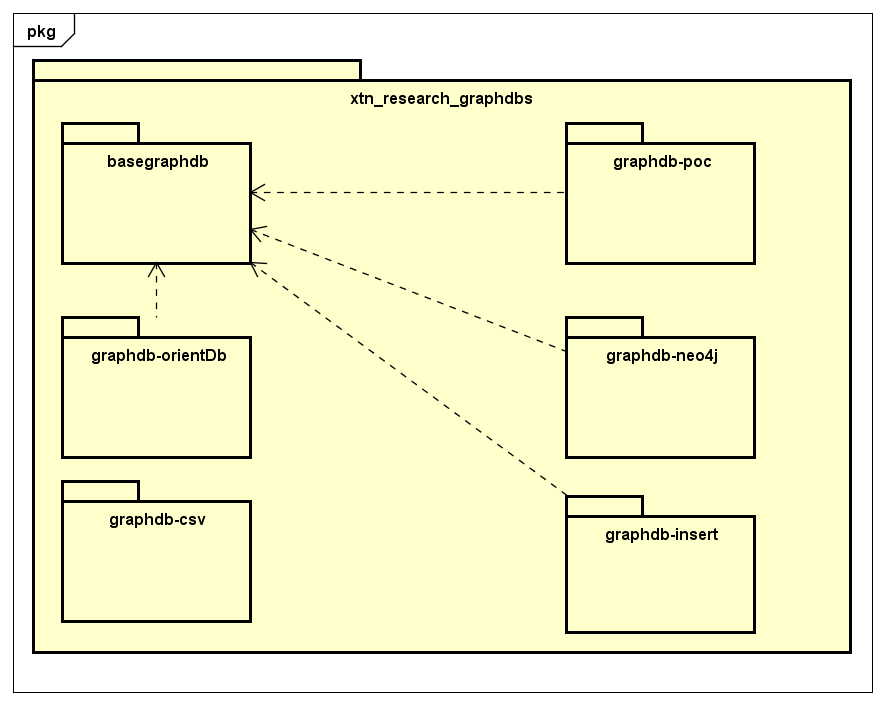
\includegraphics[scale=0.70]{diagram/img/packages.png}
	\caption{Packages}
\end{figure}

\subsubsection{basegraphdb}
Basegraphdb \'e il progetto cui contiene le varie interfacce comuni tra cui la classe \textit{ReputationController} e la classe \textit{Transaction}.
\textit{ReputationController} \'e l'interfaccia comune per gestire la reputazione delle varie entit\'a presente nei vari Database, ogni implementazione, quindi sia graphdb-neo4j, sia graphdb-orientDb che qualsiasi altra futura implementazione, ha all'interno una classe che la implementer\'a. \textit{Transaction} invece \'e una classe concreta che rappresenta una transazione indipendentemente da che implementazione di un qualsiasi database si voglia usare, l' oggetto \textit{Transaction} \'e costruito tramite l'oggetto \textit{TransactionBuilder} visto i molti parametri necessari.

\subsubsection{graphdb-orientdb}
Graphdb-orientDb \'e il progetto per la gestione della reputazione tramite OrientDB, esso ha all'interno una classe chiamata \textit{ReputationControllerOrientDb} che implementa la classe base \textit{ReputationController} contenuta nel package \textit{basegraphdb} descritta precedentemente. Questa implementazione usa Tinkerpop/BluePrints come astrazione per la gestione delle chiamate REST per l'aggiunta, modifica e interrogazione del database.

\subsubsection{graphdb-neo4j}
Graphdb-neo4j \'e il progetto per la gestione della reputazione tramite Neo4j, esso ha all'interno una classe chiamata \textit{ReputationControllerNeo4j} che implementa la classe base \textit{ReputationController} contenuta nel package \textit{basegraphdb} descritta precedentemente. Questa implementazione usa Spring Data Neo4j come astrazione per per la gestione delle chiamate REST per l'aggiunta, modifica e interrogazione del database tramite semplici annotazioni. All'interno del packag, inoltre, sono presenti tutte le classi necessarie a Spring Data per la generazione di codice sorgente come le varie classi annotate come textit{@NodeEntity} che rappresentano i nodi del grafo, oppure le varie Repository per la gestione dell'input/output del database.
Le classi annotate come \textit{@NodeEntity,@RelationshipEntity} non \'e stato possibile segnarle con visibilit\'a package, anche se sarebbe stato corretto, a causa di Spring Data Neo4j.

\subsubsection{graphdb-poc}
Graphdb-poc il progetto che si occupa solamente di istanziare le varie implementazioni di \textit{ReputationController} contenuto nel package textit{basegraphdb} ed eseguire i vari metodi tracciando, e stampando a video, il nome del metodo chiamato, il risultato ottenuto, il tipo di database che l'ha calcolato ed il tempo impiegato in millisecondi.
Questo progetto ha solamente una dipendenza verso l'interfaccia comune, l'onere di iniettare le varie dipendenze con le implementazioni viene lasciato totalmente a Spring, in questo modo si ha un disaccoppiamento tra il PoC e le varie implementazioni e, sopratutto, se in futuro ci fosse il bisogno di aggiungere un altra implementazione di \textit{ReputationController} non ci sarebbe bisogno di modificare il codice di questo progetto.

\subsubsection{graphdb-csv}
Graphdb-csv \'e il progetto per creare i diversi documenti csv contenenti le entit\'a per popolare i diversi tipi da database, questo progetto crea 4 diversi documenti csv nella root del progetto:
\begin{itemize}
\item{\textbf{account.csv:}} contenente una sola colonna con l'id del account, ad esempio l'IBAN di un conto bancario.
\item{\textbf{entity.csv:}} contenente una sola colonna con l'id di una entit\'a che ha stipulato un contratto con una banca, un entity pu\'o avere da 0 a n account associati a lui.
\item{\textbf{entity\textunderscore account.csv:}} contenente 2 colonne, un id di un entity e uno di un account, che rappresentano l'appartenenza di un account ad un entity.
\item{\textbf{transaction.csv:}} contenente tutte le informazioni di una transazione comprese il payee ed il payer.
\end{itemize}
Questo progetto crea i dati nel migliore di casi, cio\'e che ogni account ha sempre il suo entity associato.


\subsubsection{graphdb-insert}
Graphdb-insert \'e il progetto che dato il numero di account, entity e transazioni li crea nel modo del tutto casuale e li aggiunge nel database scelto. Questo progetto utilizza l'interfaccia comune \textit{ReputationController} per aggiungerli in modo indipendente all'implementazione usata.//
\textbf{Usare questa classe solo per aggiungere un basso numero di nodi visto che viene aggiunto un record in circa 500ms, in caso contrario \'e pi\'u efficiente generarsi il csv con il progetto descritto precedentemente ed utilizzare l'importatore csv nativo del database}

\subsection{Ambiente di test}
I test sono stati scritti sopo aver sviluppato il codice e sono stati testati solo i componenti non banali che utilizzavano solo librerie importare, per non rischiare di testare codice già testato da altri. \'E stato utilizzato Mockito per creare un mock dei repositori per facilitare i test che utilizzavano queste classi, invece per testare i repository sono state vere istanze di orientDb e Neo4j.
\subsubsection{Requisiti per eseguire i test}
\begin{itemize}
\item{Neo4j}: un istanza di neo4j con:
\begin{itemize}
\item{username:} neo4j
\item{password:} password
\item{Porta http:} http://127.0.0.1:7473
\end{itemize}
\item{OrientDB:} un istanza di orientDB
\begin{itemize}
\item{username:} admin
\item{password:} admin
\item{database:} un database chiamato \textit{xtn\textunderscore graph} con il seguente schema:
\begin{itemize}
\item{BaseAccount:} Una classe \textit{BaseAccount} astratta che estende da \textit{V}
\item{EntityId} Una classe \textit{EntityId} concreta che estende da \textit{V} e \textit{BaseAccount} che ha un campo dati di tipo String chiamato \textit{entityId}, ed esso \'e un indice di tipo unique.
\textit{AccountId} che ha un campo dati di tipo String chiamato \textit{accountId}, ed esso \'e un indice di tipo unique.
\item{OWN:} una classe chiamata \textit{OWN} che estende \textit{E}
\item{TRANSACTION}: una classe chiamata \textit{TRANSACTION} che estende \textit{E}
\end{itemize}
\item{Porta http:} http://127.0.0.1:7473
\end{itemize}
\end{itemize}




\section{Organizzazione della struttura di dati}
\section{Introduzione}
In questa sezione verr\'a descritta la struttura di base comune dei vari database.
\subsection{Nodi}
\begin{itemize}
\item{EntityId:} \'e il nodo che rappresenta una entity, un entity puo avere da 0 ad n AccountId associati a lui(ad esempio iban). Questo nodo \'e identificato con una stringa chiamata \textit{entityId}. Questo pu\'o effettuare transazioni ma non pu\'o riceverle.

\item{AccountId:} \'e il nodo che rappresenta un account, ad esempio un iban, ed \'e identificato da una stringa chiamata \textit{accountId}. Questo pu\'o effettuare e ricevere transazioni.

\end{itemize}

\subsection{Archi}
\begin{itemize}
\item{OWN:} \'e l'arco per descrivere la relazione di appartenenza, l'arco di tipo  \textit{OWN} ha origine da un EntityId verso un AccountId. Un EntityId pu\'o avere \textit{n>=0} archi di tipo \textit{OWN} come una persona pu\'o avere \textit{n>=0} iban.
\item{TRANSACTION:} \'e l'arco che rappresenta una transazione. Una transazione pu\'o avvenire sia da un EntityId verso un AccountID, sia da un AccountId verso un altro AccountId. Un AccountId oppure un EntityId pu\'o avere \textit{n>=0} archi di tipo \textit{TRANSACTION}.

\end{itemize}
\section{Manuale del PoC}
\subsection{Introduzione}
In questa sezione verranno descritte come usare le varie librerie disponibili, per analizzare i vari contratti dei metodi dell'interfaccia comune \textit{ReputationController} vedere documentazione contenuta direttamente nella classe.




\subsection{Uso della libreria utilizzando OrientDB e/o Neo4j}
Con il seguente codice viene creata un applicazione Spring Boot che potr\'a sfruttare, grazie al campo dati \textit{reputationController} che implementa \textit{ReputationController}, i metodi d'interfaccia. Il corpo del metodo run, o in generale di qualsiasi metodo evocato dell'interfaccia, \'e indipendente dal tipo di implementazione scelta.
\begin{lstlisting}
package it.ldario;

import it.ldario.graphdbneo4j.ReputationControllerNeo4j;
//import it.ldario.graphdborientDb.ReputationControllerOrientDb;
import org.springframework.beans.factory.annotation.Autowired;
import org.springframework.boot.CommandLineRunner;
import org.springframework.boot.SpringApplication;
import org.springframework.boot.autoconfigure.SpringBootApplication;

@SpringBootApplication
public class MiaClasse implements CommandLineRunner {

    public static void main(String[] args) {
        SpringApplication.run(MiaClasse.class, args);
    }
	//esplicitando il tipo verr\'a scelto, rispettivaemnte, il reputation controller di Neo4j o OrientDB
    private ReputationControllerNeo4j reputationController;
    //private ReputationControllerOrientDb reputationController;


    @Autowired
    public MiaClasse(ReputationControllerNeo4j reputationController) {
        this.reputationController = reputationController;
    }

    @Override
    public void run(String... strings) throws Exception {
        //aggiunge al database scelto(orientDB oppure Neo4j), dipende dal tipo che viene dichiarato, un entity con id Luca
        reputationController.addAccountId("Luca");

        //stampa la reputazione totale dell'entity Luca
        System.out.println(reputationController.getTotalReputation("Luca"));

        //stampa il totale delle transazioni effettuale da Luca negli ultimi 15 giorni

        System.out.println(reputationController.getAmountAccountIdInATimeRange("Luca", 15));
        //aggiunge al database scelto(orientDB oppure Neo4j), dipende dal tipo che viene dichiarato, un account con id IT123
         TransactionBuilder transactionBuilder = new TransactionBuilder();
        transactionBuilder.setCountry("Italy").setCity("San Michele delle Badesse").setAmount(100).setCurrency("Euro");
        reputationController.addTransaction("Luca","IT123",transactionBuilder.build());
        

    }
}
\end{lstlisting}


\subsection{Uso di graphdb-insert}
Con il seguente codice vengono generati ed aggiunti al database scelto, decidendo il tipo del capo dati \textit{reputationController}, 10 entity, 10 account(i 10 account hanno rispettivamente un loro entity deciso in modo casuale) e 10 transazioni con payer, payee e dati casuali.
\begin{lstlisting}
package it.ldario;


import it.ldario.graphdbinsert.GraphDbInsertImpl;
import it.ldario.graphdbneo4j.ReputationControllerNeo4j;
//import it.ldario.graphdborientDb.ReputationControllerOrientDb;
import org.springframework.beans.factory.annotation.Autowired;
import org.springframework.boot.CommandLineRunner;
import org.springframework.boot.SpringApplication;


public class MiaClasse implements CommandLineRunner {

    //esplicitando il tipo verr\'a scelto, rispettivaemnte, il reputation controller di Neo4j o OrientDB
    private ReputationControllerNeo4j reputationController;
    //private ReputationControllerOrientDb reputationController;

    public static void main(String[] args) {
        SpringApplication.run(GraphdbPocApplication.class, args);
    }

    @Autowired
    public MiaClasse(ReputationControllerNeo4j reputationController) {
        this.reputationController = reputationController;
    }

    @Override
    public void run(String... strings) throws Exception {
        GraphDbInsertImpl graphDbInsert = new GraphDbInsertImpl(10,10,10,reputationController);

    }
}
\end{lstlisting}

\subsection{Uso di graph-csv}
Con il seguente vengono cretai 3 file csv nella root del progetto, uno per le entity, uno per gli account, uno per la relazione di appartenenza tra entity e account e un altro per le transazioni. \textbf{Questo \'e il miglior modo per creare un numero elevato di dati e poi inserirli nel database scelto tramite il suo importatore csv}.

\begin{lstlisting}
package it.ldario;


import it.ldario.graphdbcsv.GeneratorCsv;
import it.ldario.graphdbcsv.GeneratorCsvRandom;
import it.ldario.graphdbneo4j.ReputationControllerNeo4j;
import org.springframework.boot.CommandLineRunner;
import org.springframework.boot.SpringApplication;

//import it.ldario.graphdborientDb.ReputationControllerOrientDb;


public class MiaClasse implements CommandLineRunner {

    //esplicitando il tipo verr\'a scelto, rispettivaemnte, il reputation controller di Neo4j o OrientDB
    private ReputationControllerNeo4j reputationController;
    //private ReputationControllerOrientDb reputationController;

    public static void main(String[] args) {
        SpringApplication.run(GraphdbPocApplication.class, args);
    }

    @Override
    public void run(String... strings) throws Exception {
        GeneratorCsv generatorCsv = new GeneratorCsvRandom(100, 100, 300);
    }
}
\end{lstlisting}

\subsubsection{Importare il csv creato su Neo4j}
Seguire i seguenti passi in ordine:
\begin{itemize}
\item{1:} Inserire tutti i csv creati nella cartella destinata all'import di Neo4j\\ \url{https://neo4j.com/developer/guide-import-csv/}{https://neo4j.com/developer/guide-import-csv/}.
\item{2:} Eseguire in ordine e singolarmente i comandi contenuti in \textit{configurationCsv/neo4j/comandi.txt}
\end{itemize}

\subsubsection{Importare il csv creato su OrientDB}
Seguire i seguenti passi in ordine:
\begin{itemize}
\item{1:} Inserire sia csv appena creati che tutte le configurazioni json in \textit{configurationCsv/orientdb/*.json} in una cartella visibile a orientdb.
\item{2:} Eseguire tutti i file di configurazione json come descritto nel punto 3 al seguente indirizzo \url{https://orientdb.com/docs/2.2/Import-from-CSV-to-a-Graph.html}{https://orientdb.com/docs/2.2/Import-from-CSV-to-a-Graph.html} e nel seguente ordine: entity,account,entity\textunderscore account, transaction.
\end{itemize}







\section{Conclusioni}

\subsection{Introduzione}
In questa sezione verranno descritti i vantaggi e svantaggi di delle basi di dati a grafo, pro e contro tra \textit{Neo4j} e \textit{OrientDB}, considerazioni emerse dalle prove effettuate ed infine considerazioni personali sia sulle tecnologie che, in generale, nelle basi di dati a grafo.

\subsection{Basi di dati a grafo}
\subsubsection{Vantaggi}
\begin{itemize}
\item{Velocit\'a:} la velocit\'a di determinate query, solitamente quelle che si riescono a ricondurre a dei grafi, \'e capace di restare indipendente dall'ampiezza del database stesso, questo succede quando la query si riduce ad eseguire banali, e indipendenti dalla ampiezza del DB, operazioni sui grafi come contare gli archi uscenti ed entranti. L'ambito anti frode si addice molto a questi tipi di query perch\'e molte operazioni si riducono al "\textit{conta quante volte la persona \textbf{A} ha fatto una determinata cosa, chiamata \textbf{B},  verso un entit\'a \textbf{B}}" dove A e B sono nodi e Z \'e l'arco che li collega.

\item{Espressivit\'a della ricerca:} se lo use case che si va a modellare \'e adatto alla natura dei grafi, l'espressivit\'a nella ricerca \'e tale che la query risulta banale anche dal punto di vista della scrittura. 

\item{Tutto \'e collegato:} se lo use case che si va a modellare e si \textit{astuti} nel organizzare i dati si ha un enorme possibilit\'a di creare ricerche che esplorano in profondit\'a il grafo date determinate condizioni. Nel ambito anti frode succede molto spesso di eseguire delle ricerche su entit\'a che hanno relazione, che pu\'o avere una cardinalit\'a \textit{n>0}, rispetto ad un altra entit\'a date delle particolari condizioni nelle relazioni. 

\end{itemize}

\subsubsection{Svantaggi}

\begin{itemize}

\item{Use case limitati:} solo pochi use case sono adatti ad essere modellati come un grafo, \'e molto rischioso prendere la decisione di modellare totalmente la propria base di dati come un grafo, anche se in quel momento il proprio use case sarebbe adatto, perch\'e in un futuro potrebbe esserci la necessit\'a di aggiungere dati,al modello, non adatti ad un database a grafo. Questo limita molto il normale ciclo di vita di un software.

\item{Tecnologia di nicchia:} essendo ancora un tecnologia di nicchia la possibilit\'a di informarsi, attraverso la community, \'e ridotta rispetto ad un altra tecnologia pi\'u diffusa come possono essere i database orientati ai documenti.


\end{itemize}


\subsection{Neo4j}

\subsubsection{PRO}

\begin{itemize}
\item{Espressivit\'a:} chyper, il linguaggio di quering proprietario di neo4j, inizialmente pu\'o spaventare, essendo completamente diverso dai linguaggi di quering che siamo abituati ad usare, ma dopo un breve periodo apprendimento risulta visivamente espressivo, facile da utilizzare e molto potente nelle ricerche sui grafi.
\item{Spring Data Neo4j:} al contrario di quella per orientDB \'e ben fatta e documentata.
\item{Import csv:} l'import tramite csv risulta molto pi\'u veloce sia come velocit\'a che come dinamica perch\'e, al contrario di orientDB, non \'e necessario creare nessun file di configurazione in json.
\end{itemize}

















\end{document}
